\section{Lambert's problem}

Lambert's problem is the boundary value problem (BVP) in the context of the
restricted two-body problem dynamics. Equation \ref{eq:lambert-bvp} models this
problem and figure \ref{fig:lambert-geometry} depicts its geometry.

\begin{equation}
    \ddot{\vec{r}} = -\frac{\mu}{r^3}\vec{r} \quad \begin{cases}
        \vec{r}(t_1) = \vec{r}_1 \\ 
        \vec{r}(t_2) = \vec{r}_2 \\ 
        \Delta t = t_2 - t_1
    \end{cases}
    \label{eq:lambert-bvp}
\end{equation}

If the initial position vector $\vec{r}_1$ is the launch position at time
$t_1$ and vector $\vec{r}_2$ is the arrival position at time $t_2$,
then it is possible to find the targeting orbit required to transfer a
spacecraft between the two.

Consider the case where the spacecraft is launched from a planetary body, like
the Earth, and is intended to reach an interloper. The ephemeris (position over
time) of the central body and the interloper are known. These can be used as the
input parameters for solving Lamber's problem for a given time of flight.

The solution to the Lambert's problem returns the values of $\vec{v_1}$ and
$\vec{v_2}$. Since the positions vectors are known, the computed velocity
vectors complete the state vectors at launch and arrival.

Once the velocity vectors are obtained, their modulus can be used to compute for
the required $\Delta v$. This is the increment in the velocity that needs to be
achieved by the propulsion system in order to insert the spacecraft into the
desired targeting orbit.

\begin{figure}[H]
    \centering
    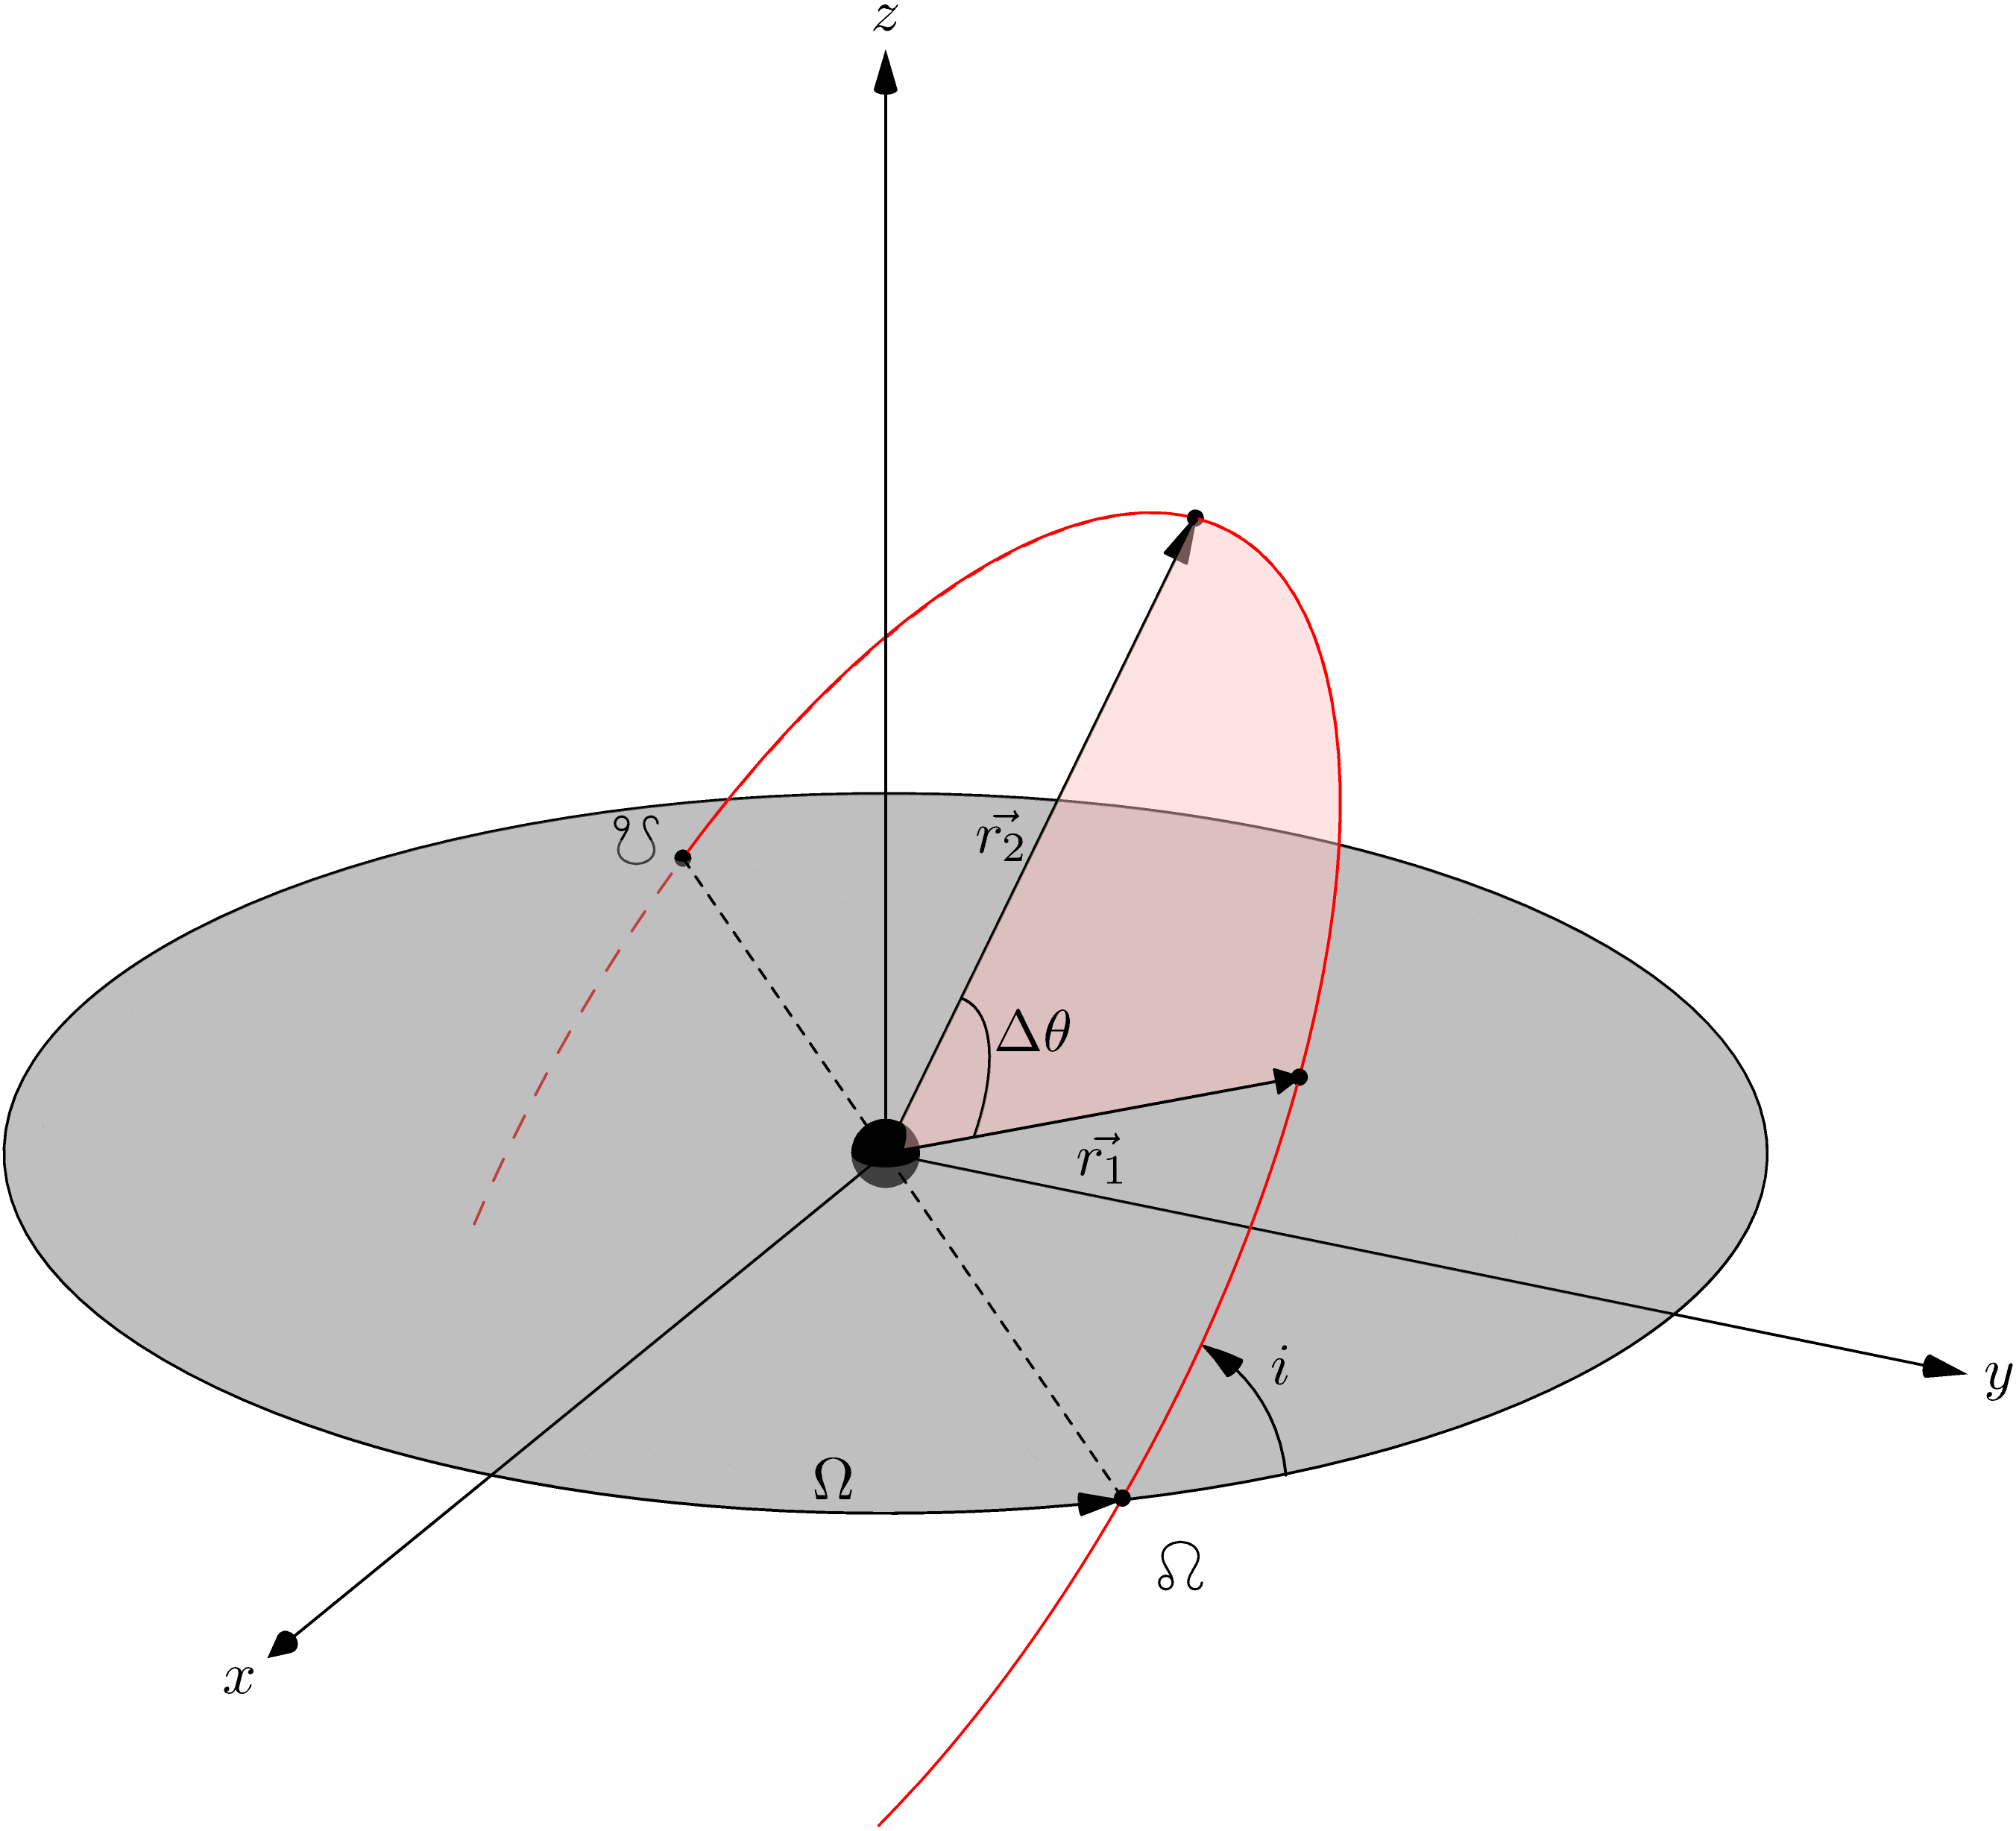
\includegraphics[width=0.75\textwidth]{lambert-problem/geometry.png}
    \caption{Lambert's problem geometry. The targeting orbit is represented by the red curve.}
    \label{fig:lambert-geometry}
\end{figure}

\subsection{Mathematical model}

Solving Lambert's problem requires numerical routines. Lots of algorithms have
been devised over the last century. The author of this document some of the most
popular ones and compared them in performance, see \cite{martinez2021}. Any
algorithm for solving Lambert's problem operates with the parameters presented
in table \ref{tab:lambert-parameters}.

\vspace{1cm}
\begin{table}[H]
    \centering
    \begin{tabular}{|c|c|}
        \hline
        Parameter & Description \\
        \hline
        $\mu$ & Gravitational parameter \\
        $\vec{r}_1$ & Initial position vector \\
        $\vec{r}_2$ & Final position vector \\
        $\Delta t$ & Time of flight \\
        $M$ & Number of desired revolutions \\
        Prograde & Inclination of the final orbit \\
        Low path & Type of path when more than two solutions are available \\
        Maxiter & Maximum number of iterations when finding a solution \\
        Atol & Absolute tolerance of the numerical routine \\
        Rtol & Relative tolerance of the numerical routien \\
        \hline
    \end{tabular}
    \caption{Parameters accepted by any Lambert's problem solver}
    \label{tab:lambert-parameters}
\end{table}

This work assumes Lambert's problem in the context of the restricted two-body
problem. This means that the only body exherting a gravitational influence is
the Sun. Thus, planetary bodies and interlopers are modeled as points with zero
mass and volume. Their gravitational influence is considered negligible, being
the only massive body the Sun. The required $\Delta v$ is modeled as an impulse.
This means that the change in the velocity is instantaneous. Perturbations are
not considered neither.

By sacrifying the accuracy of the model, the computational complexity of the
problem gets reduced. This reduces the time required to solve the problem.
Results obtained can be used as a first approximation for further refinement.
